\documentclass[11pt,twocolumn]{article}
\usepackage{graphicx}
\usepackage{pdfpages}
\usepackage{hyperref}

\hypersetup{
    colorlinks=true,
    linkcolor=blue,
    filecolor=magenta,      
    urlcolor=cyan,
}
\urlstyle{same}
\usepackage[font={small,it}]{caption}
\usepackage{fancyvrb}
\title{Analysis \& Visualization of Call Center Data using Python}
\author{John D. Bulger
\\
Karl Schmitt, PhD. (Advisor)
\\
Valparaiso University\\
}
\date{August 10, 2018}
\begin{document}
\maketitle

\begin{abstract}
\textit{The city of South Bend, Indiana operates a call center that serves as a primary point of contact for citizens.  The call center handles topics for nearly all of the city's departments.  An open data portal, maintained by the city, contains several years worth of information.  An analysis of this data was conducted using Python 3.6.  The data was 
analyzed for patterns by time of year, department, and topics with varying methods.  The cleaned, manipulated, and explored data was then developed into an 
interactive dashboard using the Bokeh library.  In doing so, an interactive HTML file will be distributed to the city, which can then be utilized, modified, and possibly connected 
directly to the data source}.
\end{abstract}

\section{Introduction}
The city of South Bend, located in northern Indiana, established a citizen-accessible call center in February 2013.  The call center handles calls from citizens regarding almost every aspect of city interaction, including waste pick-up and removal, water billing and disconnections, 
and code enforcement.  By serving as a central hub for communication, the call center is able to consolidate much of the data regarding citizen/consumer issues.  
Much of this data is available on South Bend's open data portal at \href{https://data-southbend.opendata.arcgis.com}{https://data-southbend.opendata.arcgis.com}.  The guiding questions for this analysis included seeking patterns and statistics on call volume and duration by timeframe, department, and topics.  The city has used several services/formats for data collection, resulting in data sets from differing time periods having different attributes and formats.  For most of the in-depth topic analysis, the most current format was used.

	\subsection{Prior Work}




	\subsection{Goals \& Desired Results}



\section{Methods}

%Overview of some data and Python here.

	\subsection{Loading Data}



	\subsection{Cleaning Data}


	\subsection{Data Preprocessing}



	\subsection{Discuss packages and analysis plan of attack???}



\section{Analysis}

	\subsection{Calls by Month}



	\subsection{Calls by Day}



	\subsection{Calls by Department}



	\subsection{Calls by Topic}


	\subsection{Final Dashboard}

After completion of the above analysis, the final dashboard was constructed.  Each chart in this dashboard stems from a question or interest identified by the city analysts.  The Bokeh package was used to create interactive visualizations, and allowed the final product to be conveniently packaged into a HTML file and sent to the call center management.  In all, the dashboard includes visualizations of:

\begin{itemize}
  \item{Pie chart of total call time by department}
  \item{Histogram of call volume by day of week, overlaid, with legend providing hide/show capabilities}
  \item{Bar chart of topics with longest average call duration}
  \item{Bar chart of topics with shortest average call duration}
  \item{Jitterplot of call volume by topic within top departments}
  \item{Bar chart of call volume by month}
\end{itemize}

These charts all utilize various implementation of Bokeh tools, such as HoverTool, BoxZoom, Pan, and checkbox interactivity.  By incorporating these interactions into the dashboard, the result is a more dynamic, engaging product that is simple to interact with for employees outside of the technical fields.  An image of the final dashboard can be found at the end of this paper, while a live link can be followed \href{https://jdbul33.github.io/311_Call_Dashboard.html}{here}.


\section{Discussion}


\section{Conclusions}

In summary, this analysis and presentation of data trends can be viewed as a successful high-level exploration.  Trends and points emerged from this analysis that will surely be of interest to call center management, while more insights can surely be found while interacting with the visualization dashboard.  For the city, this study should serve to identify areas of business interest within the context of these findings, which could then warrant further exploration with more specific questions.  For example, the city may want to see day-of-week trends for a specific topic, or they may seek to see how the number of calls queued relate to the number of calls abandoned.  These more specific questions would necessarily arise from a specific business need, which could perhaps be identified from this study.

	\subsection{Opportunities for Further Work}

Several paths for further work on this topic exist; however, the exact approach depends on the city's desires.  One approach would be to obtain staffing and scheduling information for the call center and use simulation and optimization techniques to evaluate staffing levels and efficiency.  Another approach would be to develop another dashboard, or perhaps modify the current one, to interact directly with the call center's data source.  This would allow a live, current view of trending topics and departments.  Such a tool could allow call center management to be agile and preemptive regarding emerging trends.



\begin{thebibliography}{6}
	
\bibitem{}


\end{thebibliography}

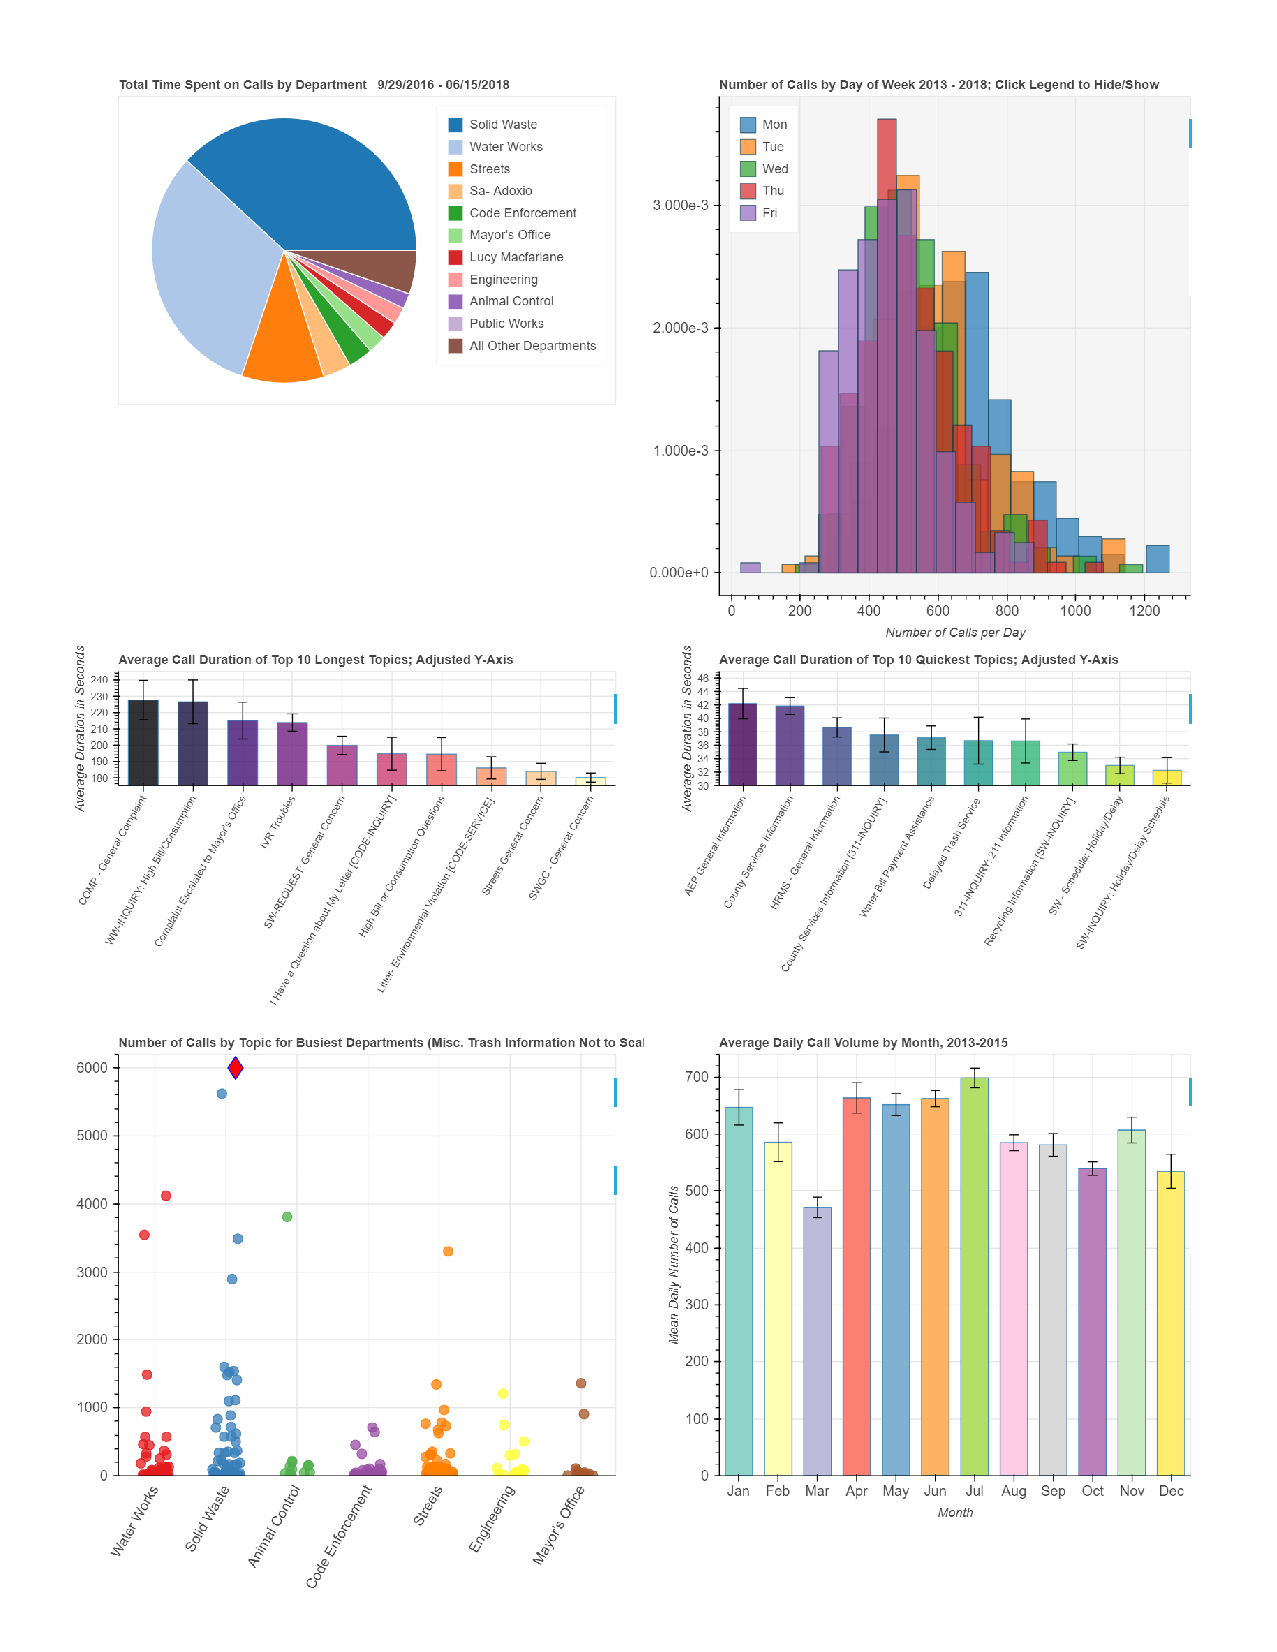
\includepdf[pages=-]{311CallCenterDashboard}



\end{document}

